\section{Case Study: UGV Sensor Resilience}
\label{s:rover}

\xpkm{This section describes details of the rover, including figures, and discusses
details of its simulation, including sensor operation and the obstacle avoidance control
algorithm. Later, we'll refer back to this algorithm when explaining side placement is likely
due to serpentine motion.}

\xpkm{Do we want to include figure and discussion of the physical rover?
Seeing the connection to real robots usually helps assure the reader that
the study is relevant to the real world.  On the other hand, we don't yet 
have any results of physical experiments.  I suppose we can say that is the
next step of this study?}

%%%%%%%%%%%%%%%%%%%%%%%%%

%\jmm{We next conduct a case study employing a commercially available robot using prebuilt control/sensor algorithms from the ROS/Gazebo Community.  
%
To demonstrate Evo-ROS on a problem of current research interest, we conducted a case study to optimize sensor placement 
on a commercially available UGV using prebuilt control/sensor algorithms from the ROS/Gazebo community.
Figure~\ref{real_rover} shows the target UGV, the Erle-Rover, a car-like robot controlled by ROS~\cite{erle.rover.main}.  
%
Erle Robotics has made available a simulated model of this platform, shown in Figure~\ref{sim_rover}.  
%
The simulated model matches the dimensions and mechanical capabilities of the physical rover, which is
%
% Control is handled through an embedded Linux computer, the Erle-Brain3.
% , that fully supports ROS and ROS 2.0.  
%
% The Erle-Brain3 seamlessly integrates the sensors and power electronics required to perform fully autonomous missions on either ground or aerial vehicles. 
% %
% Physically, the rover 
is 32.5 X 46.5 X 14.5cm with a wheel base of 33.4cm. 
%
As shown in Figure~\ref{msu_rover}, we have augmented our rover with a mounting board to hold
sensors, instruments, and battery packs. To protect the on-board electronics from impact, a roll cage has also been installed. 
%Our future work will involve validating our finding on this physical platform. 
This platform enables the investigation of several 
questions related to resiliency, including optimal sensor placement, discovery of 
execution modes for different conditions, and unwanted feature interaction.
% , and resilience to unfavorable or uncertain conditions. 
%
%We believe that work on such a platform will be directly beneficial to full scale autonomous vehicles.
%%%%%%%%%%%%%%%%%%%%%%%%%

%%%%%%%%%%%%%%%%%%%%%%%%%
%\vspace{-0.1in}
\paragraph{Sensor Placement}
We conducted several preliminary experiments where we allowed the number of sensors and their 
locations to evolve; initially, placement and orientation were not required to be symmetric.
However, we observed little convergence in those runs, and so we enforced symmetry
in all subsequent runs.
Given space limitations, we present a subset of those results here.  
Specifically, all individuals are equipped with
six sonar sensors and symmetry is enforced on the 
their evolved locations and orientations, that is, they evolve as three symmetric pairs.

Figure~\ref{ga_search_space_fig} shows the valid regions of the vehicle where 
sensors can be placed, limited by the 
% Six sensors are placed on the rover with left/right symmetry enforced.  
%
physical configuration of the existing Erle-Rover.
%
Sensors are constrained to the outer 5cm on the front half of the rover.  
%
For this study, the controller does not drive in reverse so we do not consider placement on the rear half of the rover.  
%
Sensor orientation is also constrained to orient sensing regions to the front or sides of the rover.  
Failure models for sensors are described below.
%%%%%%%%%%%%%%%%%%%%%%%%%
\vspace{-0.1in}
\begin{figure}[ht]
	\centering
    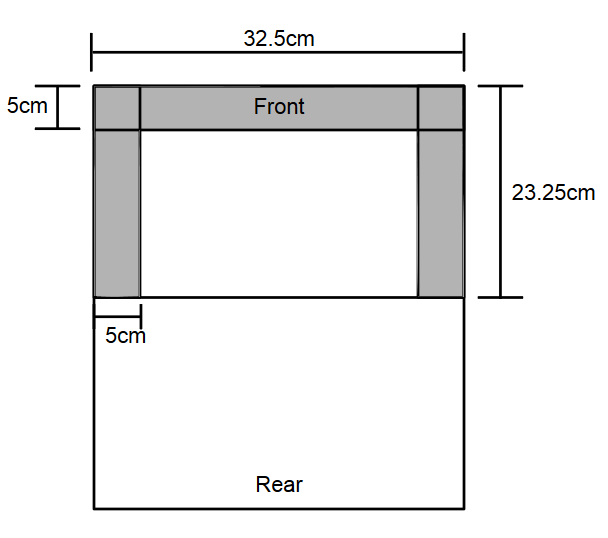
\includegraphics[width=0.32\textwidth]{Figures/sensor_placement_shaded.png}
    \vspace{-0.2in}
    \caption{Sensors can be placed on the outer 5cm on the front half of the robot in the shaded region.}
    \label{ga_search_space_fig}
    \vspace{-0.1in}
\end{figure}

%%%%%%%%%%%%%%%%%%%%%%%%%
\paragraph{Control Hardware}
Rover control is handled through a combination of Ardupilot waypoint navigation and an override when obstacle avoidance is required.  
%
Incorporating Ardupilot requires adding the {\tt arupilot\_sitl\_gazebo\_plugin}~\cite{ardupilot.sitl.plugin} to the simulation environment.  
%
Doing so ensures proper interaction between a Gazebo simulation and the Ardupilot autopilot,
but forces simulations to run at Ardupilot's fixed 400Hz update rate.
%
Evo-ROS implements a step-lock mechanism at each simulation timestep, synchronizing the Gazebo simulation and Ardupilot by pausing the simulation until a new movement command is received.  
%
Evo-ROS then steps the simulation by 2.5ms and returns
new sensor measurements to Ardupilot.
%
Unlike typical Gazebo simulations where the simulator runs without waiting for commands, 
Ardupilot is the master of the simulation clock \cite{erle.simulation}. 
%
The availability of the simulated Erle-Rover model and the Ardupilot plugin provides an accurate representation of the physical rover and portability of evolved controller code between simulated and physical rovers. 
%
% This is helpful when transferring control code while assisting with the reality gap, a topic of our ongoing study.
%
We emphasize, however, that Ardupilot is not integral to Evo-ROS.  As discussed later, we are currently conducting studies that replace Ardupilot with other control software.
% \jmm{From the case study, we have identified removal of the Ardupilot stack as an area for future improvement and discuss further in Section~\ref{s:conclusions}.}
%
%Nonetheless, in future work we plan to create a custom autopilot plugin, freeing us from the 400Hz update limitation imposed by Ardupilot.
%%%%%%%%%%%%%%%%%%%%%%%%%


% \begin{figure*}[!htb]
%     \centering
    
%     \begin{subfigure}[t]{0.33\textwidth}
%         \centering
%         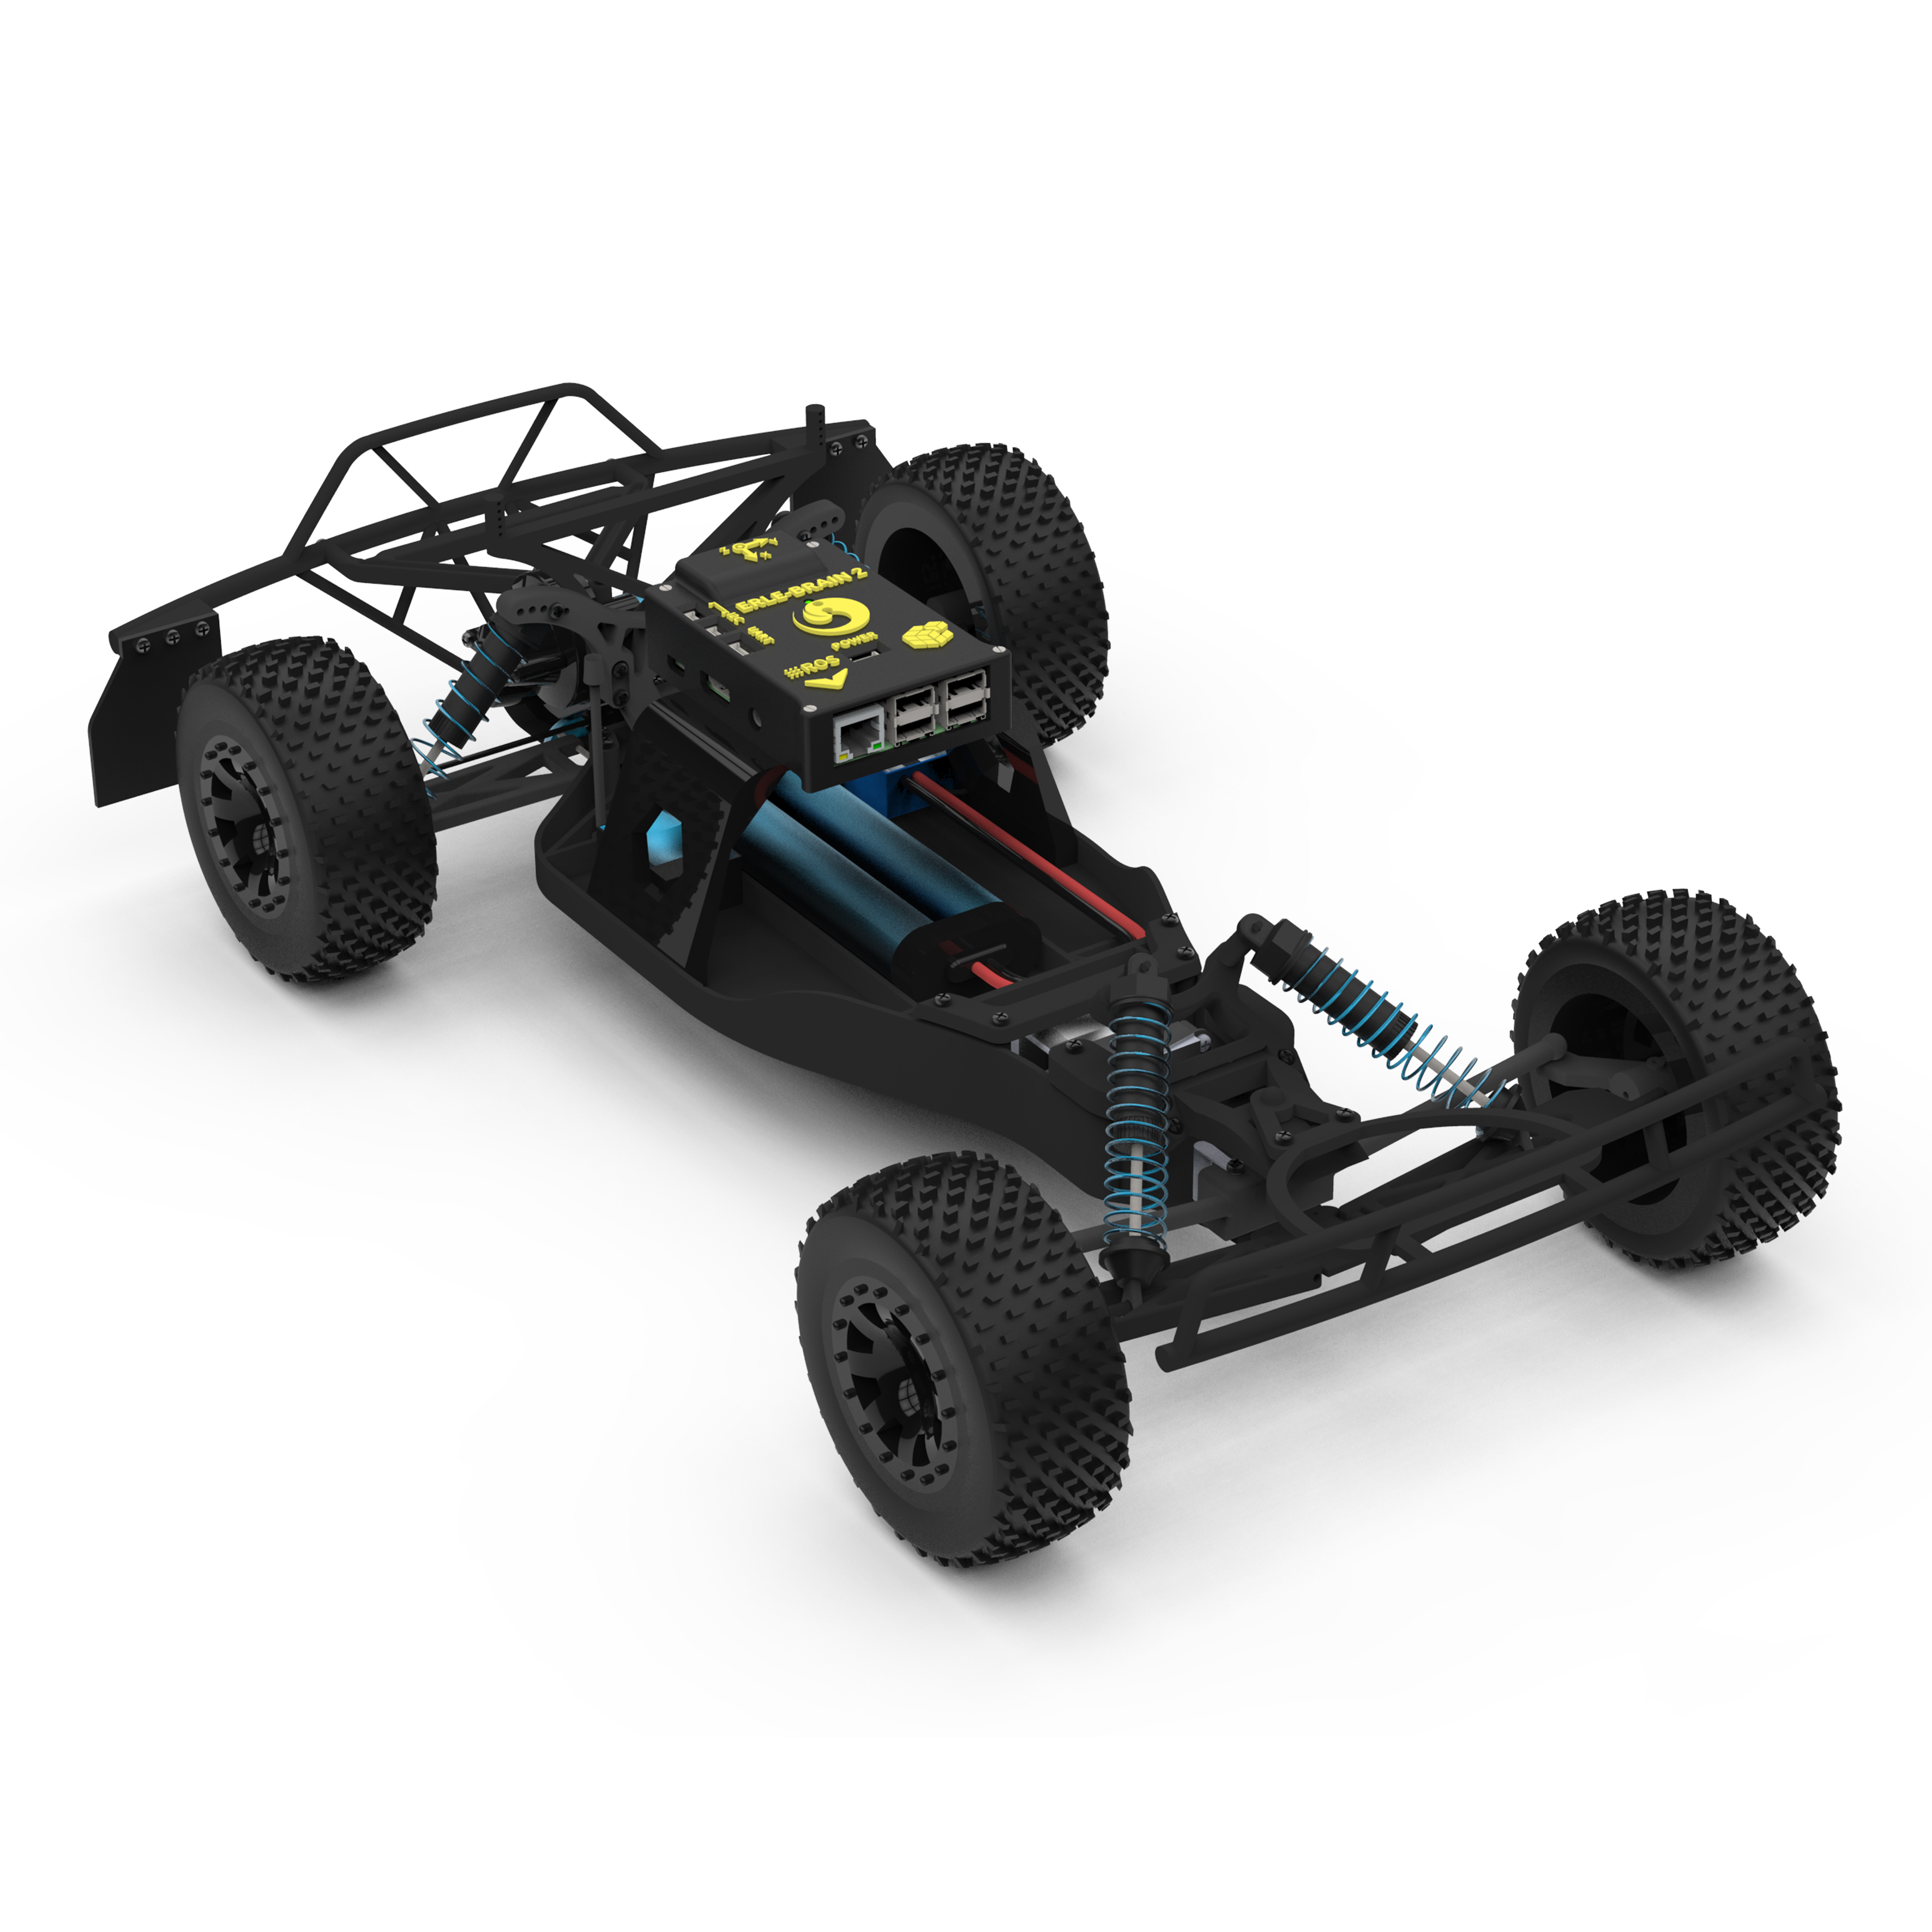
\includegraphics[height=1.2in]{Figures/ErleRover.jpg}
%         \caption{Physical Erle-Rover frame}
%         \label{real_rover}
%     \end{subfigure}%
%     ~ 
%     \begin{subfigure}[t]{0.33\textwidth}
%         \centering
%         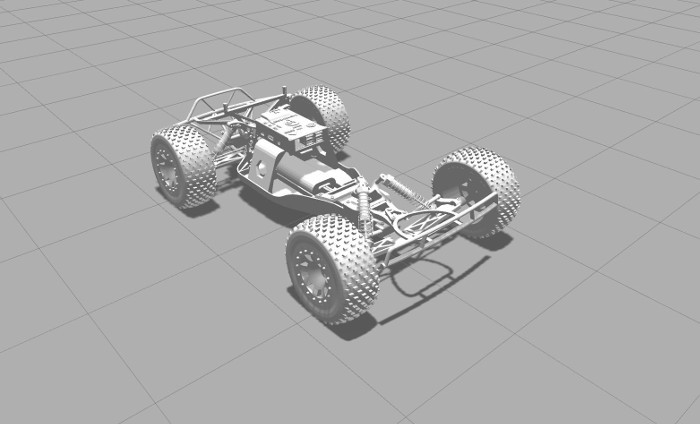
\includegraphics[height=1.2in]{Figures/rover.jpg}
%         \caption{Gazebo simulated Erle-Rover}
%         \label{sim_rover}
%     \end{subfigure}
%     ~
%      \begin{subfigure}[t]{0.33\textwidth}
%         \centering
%         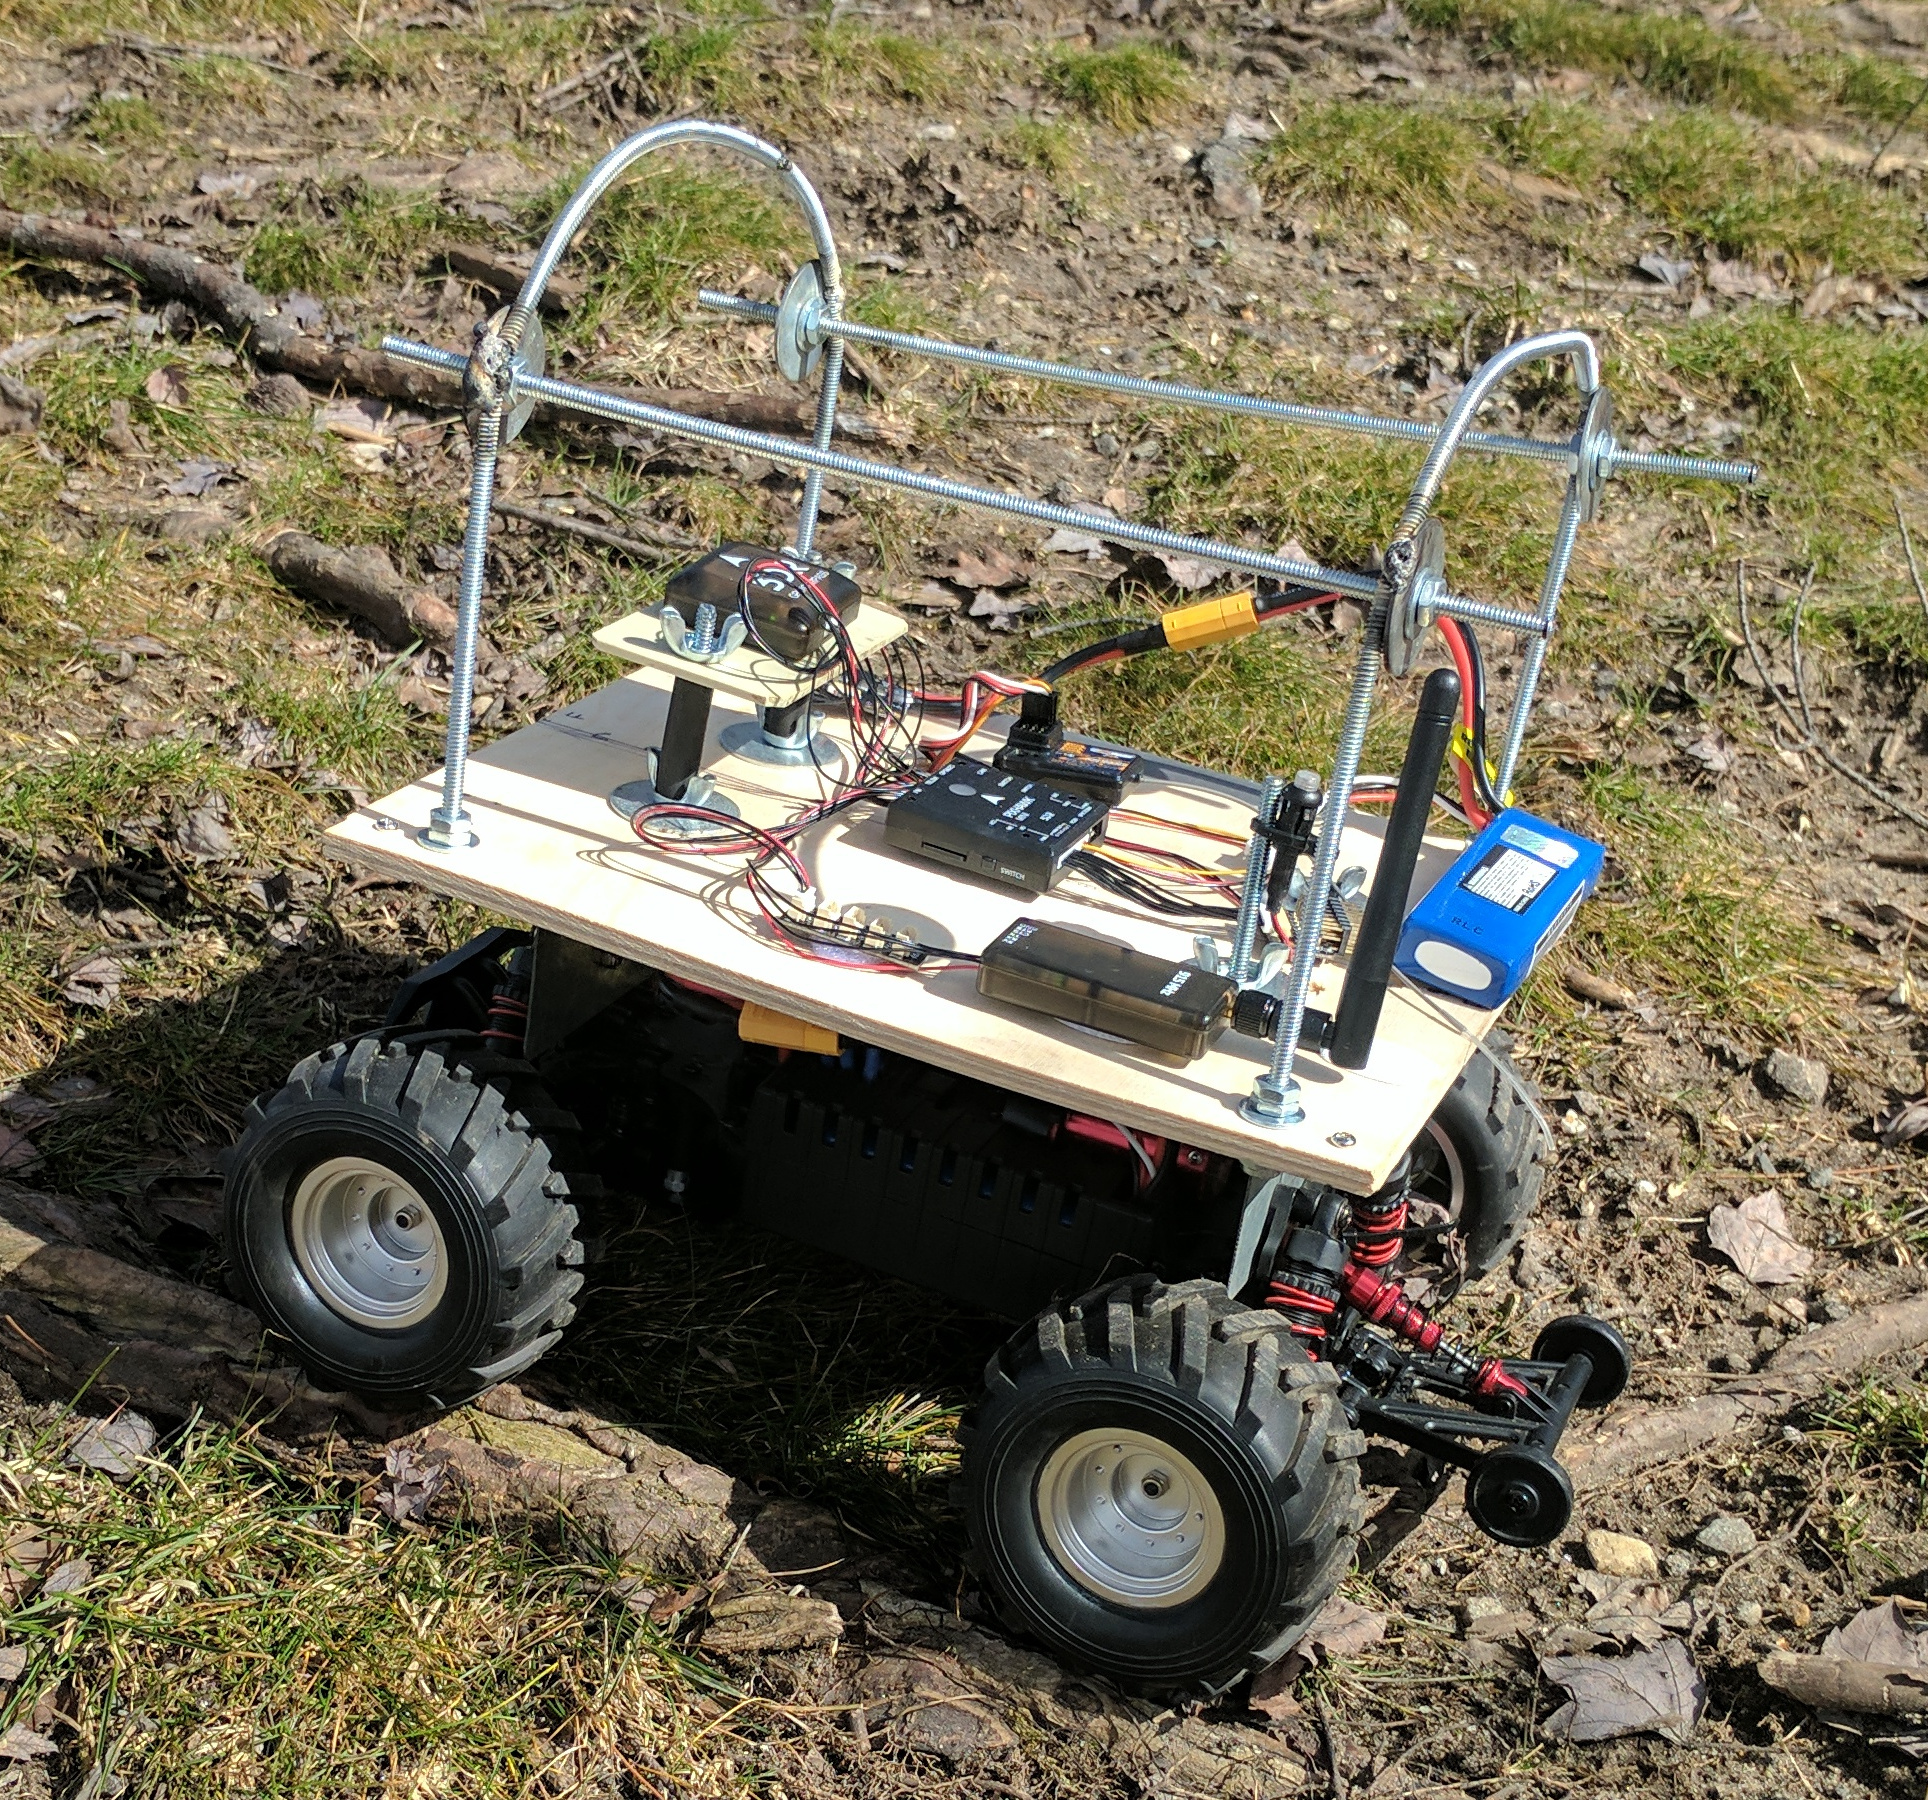
\includegraphics[height=1.2in]{Figures/real_rover_cropped.jpg}
%         \caption{Physical rover frame equipped with sensor board, sensors, and a roll cage}
%         \label{msu_rover}
%     \end{subfigure}
%     \caption{ }
%     \label{rover_pics}
% \end{figure*}

%%%%%%%%%%%%%%%%%%%%%%%%%

\xpkm{Minor point.  Following text mentions mazes.  We need to have introduced that term earlier when
mentioning environments.}

\vspace{-0.08in}
\paragraph{Evaluation}
Figure~\ref{waypoint_mission_fig} depicts one of the three environments
used to evaluate individuals.  
%
% \jmm{
Environments are specified in a Gazebo specific file format, facilitating reuse between experiments.
% }
%
Each rover carries out a pre-defined waypoint following mission, in two phases. 
%
First, a rover navigates through the waypoints within the environment,
eventually returning to the starting location. 
%
If the rover successfully completes the first phase, it then must navigate the waypoints in reverse order, finally returning home again. 
%
Having two phases is intended to avoid
sensor configurations from becoming overfit to missions favoring turns in one direction.
%
In addition, the direction of the first phase
is selected randomly to deter sensor configurations from ``memorizing'' the route. 
%%%%%%%%%%%%%%%%%%%%%%%%%

\vspace{-0.05in}
\begin{figure}[ht]
\centering
    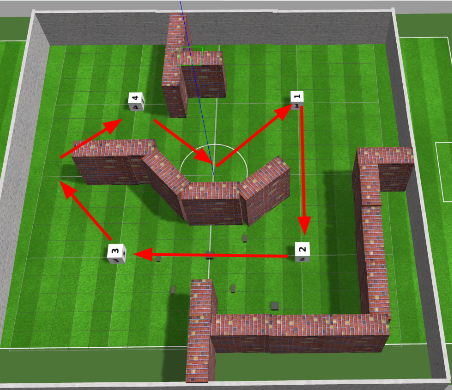
\includegraphics[width=0.4\textwidth]{Figures/waypoint_mission.PNG}
    \vspace{-0.1in}
    \caption{A sample first phase of a mission path consisting of four waypoints in oriented around a home location.}
    \label{waypoint_mission_fig}
    \vspace{-0.1in}
\end{figure}
%%%%%%%%%%%%%%%%%%%%%%%%%

%%%%%%%%%%%%%%%%%%%%%%%%%
\paragraph{Fitness}
Fitness reflects individual performance in three different environments, specifically:
\begin{equation}
fit = \sum_{n=1}^{3} (1 + perc\_complete)^2 + C * (1 + perc\_time\_remaining)^2
\label{eq:fitness}
\end{equation}

\noindent
where $perc\_compelete$ represents the percentage of
mission completed, $C$ is either 1 or 0
indicating whether or not the mission was completed, and
$perc\_time\_remaining$ indicates how much of the allotted
time remained at the completion of the mission.

%%%%%%%%%%%%%%%%%%%%%%%%%

%%%%%%%%%%%%%%%%%%%%%%%%%
%\vspace{-0.1in}
\paragraph{Control}
The control strategy is split into two different modes,~(1) a waypoint following mode
encoded in Ardupilot and~(2) a ROS-based obstacle avoidance mode. 
%
Both modes pass commands to the simulated rover via UDP sockets maintained by Ardupilot. 
%
By default, the waypoint following algorithm
governs navigation when no obstacles are detected by sensors~\cite{Ardupilot.Auto}.
%
% The rover follows a pre-programmed mission script stored in the autopilot composed of navigation commands (i.e., waypoints)
%
Ardupilot navigates between waypoints using a serpentine driving behavior, sweeping the front of the rover through a 60 degree arc as it moves forward, rather than following a straight line. 
%
When at least one sensor detects an obstacle within a threshold distance from the vehicle,
the obstacle avoidance mode preempts the waypoint following algorithm.
%
Obstacle avoidance is
implemented by switching Ardupilot into ``Manual'' mode and sending movement commands from a ROS script.
%
Once the obstacle is cleared, waypoint navigation resumes.  
%%%%%%%%%%%%%%%%%%%%%%%%%

%%%%%%%%%%%%%%%%%%%%%%%%%
\xpkm{This paragraph will be hard for the reader to follow.}
\xjmm{Again, do we need such a technical description?  The previous paragraph explains the two command modes.  I don't know that a reader cares so much about the specific implementation details.  I moved the final sentence of this paragraph to the one above and suggest that we delete the following paragraph.}



The command flow for operating in these two modes can be seen in the bottom half of Figure~\ref{evo_ros_diagram}. In the waypoint following mode, commands are generated by the APMRover process within Ardupilot. In the obstacle avoidance mode, commands are generated by the navigation controller on the rover. These commands are passed through the MAVROS process so that they can be translated to follow the MAVLink protocol. Regardless of the source, the MAVProxy process is responsible for the communication of the commands to either a physical rover or, in our case, a simulated one.
% The bottom half of Figure~\ref{evo_ros_diagram} shows the configuration of 
% these two command modes.
%

%
% Within Ardupilot, waypoint following commands are generated in the 
% % APMRover process and passed to MAVProxy,
%
% which translates these, and override commands, into rover-specific 
% movement commands~(e.g. accelerate, turn). %
% Obstacle avoidance controls are generated in the rover's ROS-based Navigation 
% Controller and passed to a MAVROS process.  
%
% Commands are then sent to MAVProxy along with a command to switch into ``Manual'' mode preempting waypoint navigation for obstacle avoidance.  
%%%%%%%%%%%%%%%%%%%%%%%%%

%%%%%%%%%%%%%%%%%%%%%%%%%
Obstacle avoidance commands are generated using a weighted voting algorithm.  
%
Each sensor that detects an obstacle casts a vote to turn either left or right, depending on the orientation of the sensor. 
%
For example, if a sensor on the front of the vehicle
and angled slightly left detects an obstacle, it would vote to turn right. 
%
Each vote is weighted based on the proximity of the detected object.
%
% A sensor detecting an object two meters away will impact the voting result more than a sensor detecting an object four meters away. 
%
After each sensor has cast its vote, the right and left totals are calculated.
%  along with the difference. 
%
A small difference, with both left and right votes above a certain threshold,
indicates that an object is directly in front of the rover.  
%
The default response is to navigate left around the object. 
%
Otherwise, turning direction is determined by the sign of the difference between the left/right votes, negative indicating a left turn and positive indicating right. 
%
The strength, or sharpness, of the turn is determined by the following equation:
%\vspace{-0.05in}
\begin{equation}
turn\_strength = 1 - \frac{(max\_range - \left | {\sum_{i=0}^{6}w_i * d_i} \right |)}{max\_range}
\label{eq:turn}
%\vspace{-0.05in}
\end{equation}
\noindent
where $max\_range$ is the maximum detection range for the sensor,
$w_i$ is the weight and $d_i$ is the turn direction vote for the $i^{th}$ sensor.  
%
The summation takes into account all voting sensors.
%
%
If $turn\_strength$ is 1.0 the rover will turn as sharply as possible.
%
As $turn\_strength$ approaches 0 the turn becomes more gradual.
%
After an obstacle has been avoided and no sensors report collision threats, 
the autopilot returns to the waypoint following behavior. 
%%%%%%%%%%%%%%%%%%%%%%%%%

%%%%%%%%%%%%%%%%%%%%%%%%%
% \jmm{ TODO: Cut? 
% While the work done in this study focuses on the performance of sensor configurations in a simulated environment, a physical platform, seen in figure \ref{msu_rover}, modeled after the Erle-Rover has been developed and built. This platform rover frame has dimensions of 23.4 x 32.5 x 16cm. Additionally, it is equipped with a mounting board for required sensors, instruments, and battery packs. To protect the on-board electronics from impact, a roll cage has also been installed. Our future work will involve validating our finding on this physical platform. 
% }
%%%%%%%%%%%%%%%%%%%%%%%%%

